\documentclass[a4paper]{article}
\usepackage[utf8]{inputenc}
\usepackage[russian,english]{babel}
\usepackage[T2A]{fontenc}
\usepackage[left=10mm, top=20mm, right=18mm, bottom=15mm, footskip=10mm]{geometry}
\usepackage{indentfirst}
\usepackage{amsmath,amssymb}
\usepackage[italicdiff]{physics}
\usepackage{graphicx}
\graphicspath{{images/}}
\DeclareGraphicsExtensions{.pdf,.png,.jpg}
\usepackage{wrapfig}
\usepackage{float}
\usepackage{subcaption}
\usepackage{enumitem}
\usepackage{caption}
\usepackage{array}
\captionsetup[figure]{name=Рисунок}
\captionsetup[table]{name=Таблица}

\title{\underline{Отчет о выполненой лабораторной работе 4.7.1}}
\author{Воронин Денис, Б04-407}

\begin{document}

\maketitle

\begin{center}
\textbf{\Large Двойное лучепреломление}
\end{center}

\textbf{Цель работы:} изучение зависимости показателя преломления
необыкновенной волны от направления в двоякопреломляющем кристалле; определение главных показателей преломления в кристалле.

\textbf{В работе используются:} гелий-неоновый лазер, вращающийся столик с неподвижным лимбом, призма из исландского шпата, поляроид.

\section{Аннотация}

По окончанни работы хотим полуить \textbf{преломляющий угол призмы A} и определить \textbf{главные показатели преломления $n_0$ и $n_e$} исландского 
шпат, сняв для обыкновенного и необыкновенного лучей зависимость координаты преломленного луча от координаты отраженного.

\section{Теоретические сведения}

\begin{wrapfigure}{l}{0.5\textwidth}
  \centering
  
\includegraphics[width=0.3\textwidth]{pi1.png}
  \caption{Двойное лучепреломление: расщепление луча на обыкновенный(o) и необыкновенный(e)
}
  \label{fig:example}
\end{wrapfigure}

Рассмотрим особенности распространения электромагнитных волн в анизотропных средах, то есть веществах, обладающих выделенными направлениями.

При падении света на некоторые кристаллы  (исландский шпат) луч расщепляется на два луча. Один из них, следующий обычным законом преломления, называется \textbf{обыкновенным} (обозначается символом <<$o$>> = \textit{ordinary}), а второй — \textbf{необыкновенным} (обозначается символом <<$e$>> = \textit{extraordinary}) (рис. 1)

Описанное явление было обнаружено в 1669~г. на кристалле исландского шпата . Нидерландский физик связал явление с тем, что обыкновенный и необыкновенный лучи имеют разную поляризацию, и ввёл понятие оптической оси кристалла.

Явление расщепления одного луча на два, различающихся по свойствам, называется \par \textbf{двойным лучепреломлением}.

В кристаллах существуют оси, вдоль которых обыкновенный и необыкновенный лучи распространяются вместе, не разделяясь и с одинаковой скоростью. В общем случае таких осей две. Соответствующие направления называются \textbf{оптическими осями кристалла}.

В некоторых кристаллах оптические оси совпадают, так что фактически он обладает единственной оптической осью. В этом случае кристалл называется \textbf{одноосным}.

\begin{wrapfigure}{l}{0.3\textwidth}
  \centering
  
\includegraphics[width=0.2\textwidth]{pi2.png}
  \caption{Расположение
}
  \label{fig:example}
\end{wrapfigure}

Для обыкновенного луча показатель преломления не зависит от направления распространения, а для необыкновенного — зависит.

Распространение электромагнитных волн описывается уравнениями Максвелла, которые в отсутствие электрических зарядов и токов имеют вид
\begin{equation}
\operatorname{rot} \vec{H} = \frac{1}{c} \frac{\partial \vec{D}}{\partial t}, \qquad
\operatorname{rot} \vec{E} = -\frac{1}{c} \frac{\partial \vec{H}}{\partial t}.
\label{eq:maxwell_no_sources}
\end{equation}

% \begin{wrapfigure}{l}{0.3\textwidth}
%   \centering
%   
\includegraphics[width=0.2\textwidth]{pi2.png}
%   \caption{Расположение
% }
%   \label{fig:example}
% \end{wrapfigure}

Условия, при которых в одноосных кристаллах могут распространяться плоские монохроматические волы вида:

\begin{equation}
\vec{E} = \vec{E}_0 e^{i(\omega t - \vec{k}\cdot\vec{r})}, \quad
\vec{H} = \vec{H}_0 e^{i(\omega t - \vec{k}\cdot\vec{r})}, \quad
\vec{D} = \vec{D}_0 e^{i(\omega t - \vec{k}\cdot\vec{r})},
\label{eq:plane_wave_fields}
\end{equation}

Подставив их в уравнения Максвелла получим (D, H, k - взаимно перпендикулярны):

\begin{equation}
\vec{D} = -\frac{c}{\omega} \, \vec{k} \times \vec{H},
\label{eq:D_from_k_H}
\end{equation}
\begin{equation}
\vec{H} = \frac{c}{\omega} \, \vec{k} \times \vec{E}.
\label{eq:H_from_k_E}
\end{equation}

% \newpage

\begin{figure}[h]
    \centering
    
\includegraphics[width=0.6\textwidth]{pi3.png}
    \caption{Обыкновенная (а) и необыкновенная (б) волны и положение
основных векторов в них. Плоскость рисунка главное сечение}
    \label{fig:example}
\end{figure}

Фазовые скорости волн обыкновенной и необыкновенной:

\begin{equation}
v_o = \frac{c}{\sqrt{\varepsilon_\perp}} = \frac{c}{n_o},
\label{eq:ordinary_velocity}
\end{equation}

\begin{equation}
v_e = \frac{c}{\sqrt{\varepsilon}} = \frac{c}{n(\theta)}, \qquad
\text{где } \varepsilon = \frac{1}{\dfrac{\sin^2\theta}{\varepsilon_\parallel} + \dfrac{\cos^2\theta}{\varepsilon_\perp}}.
\label{eq:extraordinary_velocity_full}
\end{equation}

В исследуемой призме ось кристалла лежит в плоскости, параллельной верхней грани призмы, причём она параллельна входной грани призмы (длинному катету). 
При этом в обыкновенной волне вектор $\vec{D}_o$ перпендикулярен верхней грани призмы, а в необыкновенной волне вектор $\vec{D}_e$ параллелен верхней грани.

\begin{figure}[h]
    \centering
    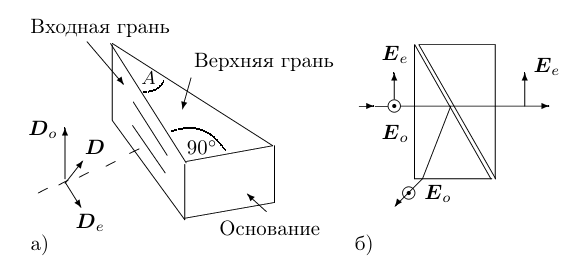
\includegraphics[width=0.6\textwidth]{pi4.png}
    \caption{ а) Исследуемая призма из исландского шпата. Штриховкой указано
направление оптической оси кристалла. б) Ход лучей в поляризационной
призме}
    \label{fig:example}
\end{figure}

\begin{wrapfigure}{l}{0.3\textwidth}
  \centering
  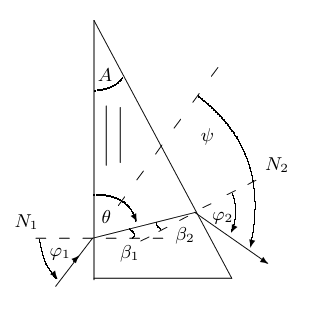
\includegraphics[width=0.3\textwidth]{pi5.png}
  \caption{Ход лучей в призме
}
  \label{fig:example}
\end{wrapfigure}

$A = \beta_1 + \beta_2$. Учитывая, что угол преломления $\beta_1$ связан с углом $\theta$ между осью кристалла и волновой нормалью N соотношением $\theta + \beta_1 = \frac{\pi}{2}$,
находим n и $\theta$:

% \begin{wrapfigure}{l}{0.3\textwidth}
%   \centering
%   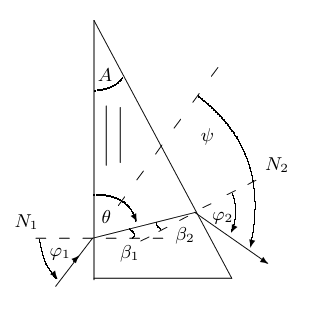
\includegraphics[width=0.3\textwidth]{pi5.png}
%   \caption{Ход лучей в призме
% }
%   \label{fig:example}
% \end{wrapfigure}

\begin{equation}
n = \frac{1}{\sin A} \sqrt{ \sin^2\varphi_1 + \sin^2\varphi_2 + 2 \sin\varphi_1 \sin\varphi_2 \cos A },
\label{eq:refractive_index_general}
\end{equation}
\begin{equation}
\cos\theta = \frac{\sin\varphi_1}{n}.
\label{eq:cos_theta}
\end{equation}


Для обыкновенной волны $n$ не будет зависеть от угла $\theta$, а для необыкновенной волны зависимость $n$ от $\theta$ должна описываться выражением~\eqref{eq:refractive_index_general}.

Показатель преломления призмы из изотропного материала удобно находить по углу наименьшего отклонения луча от первоначального направления. Угол отклонения луча призмой ($\psi$ на рис.~2) минимален для симметричного хода лучей, т.е. когда $\varphi_1 = \varphi_2$. Тогда показатель преломления можно рассчитать по формуле
\begin{equation}
n = \frac{\sin\left( \dfrac{\psi_m + A}{2} \right)}{\sin\left( \dfrac{A}{2} \right)},
\label{eq:refractive_index_min_deviation}
\end{equation}
где $\psi_m$ — угол наименьшего отклонения.

\section{Лабораторная установка}

\begin{wrapfigure}{l}{0.6\textwidth}
  \centering
  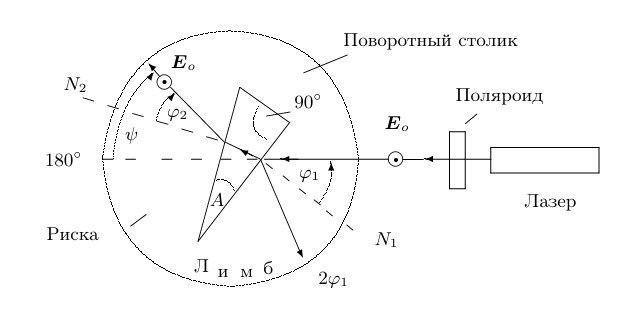
\includegraphics[width=0.6\textwidth]{pi6.png}
  \caption{Схема экспериментальной установки
}
  \label{fig:example}
\end{wrapfigure}

\textbf{Экспериментальная установка.} Схема экспериментальной установки изображена на рис.~6. Источником излучения служит Ne--Ne-лазер ($\lambda = 0.63~\mathrm{мкм}$). Излучение лазера поляризовано линейно за счёт наличия бристовских окошек в кювете лазера. Направление вектора $\vec{E}$ в луче можно изменять с помощью поляроида, установленного на выходе лазера. Исследуемая призма из исландского шпата закреплена в центре поворотного столика с нжным лимбом для отсчёта углов.

Преломляющий угол $A$ призмы можно рассчитать, если известны угловые координаты нормалей $N_1$ и $N_2$ к преломляющим (рабочим) граням призмы, прилегающим преломляющему углу. Грань, противолежащая преломляющему углу, называется \textbf{основанием призмы}. Штриховкой указано направление оптической оси.

Обычно ход лучей в призме таков, что и падающий, и преломлённый лучи отклоняются от нормалей в сторону основания призмы, при этом углы $\varphi_1$ и $\varphi_2$ считаются положительными.

Угол падения $\varphi_1$ определяется по положению луча, отражённого от передней (входной) грани призмы (рис.~3). Из рис.~2 можно получить связь углов $\varphi_1$ и $\varphi_2$:
\begin{equation}
\varphi_2 = A + \psi - \varphi_1,
\label{eq:angle_relation_prism}
\end{equation}
а угол $\psi$ — отклонение преломлённого луча от первоначального направления — определяется по разности отсчётов на лимбе между точками, куда попадает луч в отсутствие призмы, и точкой, куда попадает преломлённый луч.

\section{Ход работы}

\subsection{Юстировка системы}

Провели юстировку системы согласно описанию хода работы п.1.

\subsection{Измерение преломляющего угла призмы (A)}

Вращая столик с призмой и меняя стороны, на которые падал луч лазера (длинный катет, гипотенуза) провели измерения, результаты которых внесли в таблицу (погрешности возьмем равные половине цены деления шкалы на лимбе).

\par

Формула для вычисления угла A находиться по формуле:

\[ A = (2\varphi_2 - 2\varphi_1) -180 \]

Подсчитывая среднее значение и учитывая погрешность (подсчитана ниже) получим:

\[A = 38.409 \pm 0.202 \]

Формула для подсчета погрешности:

\begin{equation}
s_{n-1} = \sqrt{ \frac{1}{n-1} \sum_{i=1}^{n} \Delta x_i^2 },
\label{eq:sample_std_dev}
\end{equation}


% \begin{table}[h!]
% \centering
% \caption{Пример таблицы}
% \label{tab:example}
\begin{tabular}{|>{\raggedright\arraybackslash}p{4.5cm}|>{\raggedright\arraybackslash}p{4.5cm}|>{\raggedright\arraybackslash}p{4.5cm}|}
\hline
\textbf{Координата отраженного луча по лимбу} & \textbf{Отсчет по риске при отражения от длинного катета } & \textbf{Отсчет по риске при отражении от гипотенузы} \\
\hline
$10.0 \pm 0.5$  & $65.0 \pm 0.5$ & $283.0 \pm 0.5$ \\
\hline
$20.0 \pm 0.5$ & $70.0 \pm 0.5$ & $288.0 \pm 0.5$ \\
\hline
$30.0 \pm 0.5$ & $75.0 \pm 0.5$ & $293.5 \pm 0.5$ \\
\hline
$40.0 \pm 0.5$ & $80.0 \pm 0.5$ & $298.5 \pm 0.5$ \\
\hline
$50.0 \pm 0.5$ & $85.0 \pm 0.5$ & $303.5 \pm 0.5$ \\
\hline
$60.0 \pm 0.5$ & $90.0 \pm 0.5$ & --- \\
\hline
$70.0 \pm 0.5$ & $95.0 \pm 0.5$ & $313.5 \pm 0.5$ \\
\hline
$80.0 \pm 0.5$ & $100.0 \pm 0.5$ & $318.5 \pm 0.5$ \\
\hline
$90.0 \pm 0.5$ & $105.0 \pm 0.5$ & $323.5 \pm 0.5$ \\
\hline
$100.0 \pm 0.5$ & $110.0 \pm 0.5$ & $328.5 \pm 0.5$ \\
\hline
$110.0 \pm 0.5$ & $115.0 \pm 0.5$ & $333.5 \pm 0.5$ \\
\hline
$120.0 \pm 0.5$ & $120.0 \pm 0.5$ & $338.5 \pm 0.5$ \\
\hline
$130.0 \pm 0.5$ & $125.0 \pm 0.5$ & --- \\
\hline
$140.0 \pm 0.5$ & $130.0 \pm 0.5$ & --- \\
\hline
\end{tabular}
% \end{table}

\subsection{Определение обыкновенного и необыкновенного луча}

Настроили поляроид на минимум пропускание. В таком случае разрешенное направление E вертикально.
Получим на лимбе изображение преломленных лучей так, как показано на рис.6 (падающий и преломленный лучи отклоняются от нормалей в сторону основания призмы).
Установим поляризатор между лазером и призмой.\par 
Вращая поляризатор выяснили, что вертикально поляризованному свету соответствует необыкновенный луч, а горизонтально поляризованному соответствует обыкновенный луч. 
От первоначального положения больше отклоняется необыкновенный луч.

\subsection{Измерение главных показателей преломления}

Изменяя координату луча, отраженного от входной грани призмы, определим координаты углов преломления для обыкновенного и необыкновенного лучей. Результаты содержаться в таблице:

\begin{tabular}{|>{\raggedright\arraybackslash}p{4.5cm}|>{\raggedright\arraybackslash}p{4.5cm}|>{\raggedright\arraybackslash}p{4.5cm}|}
\hline
\textbf{Координата отраженного луча по лимбу} & \textbf{Координаты углов преломления для обыкновенного луча} & \textbf{Координаты углов преломления для необыкновенного луча} \\
\hline
$20.0 \pm 0.5$ & $202.5 \pm 0.5$ & $212.5 \pm 0.5$ \\
\hline
$30.0 \pm 0.5$ & $201.7 \pm 0.5$ & $210.0 \pm 0.5$ \\
\hline
$40.0 \pm 0.5$ & $201.0 \pm 0.5$ & $209.0 \pm 0.5$ \\
\hline
$50.0 \pm 0.5$ & $200.9 \pm 0.5$ & $208.0 \pm 0.5$ \\
\hline
$60.0 \pm 0.5$ & $200.9 \pm 0.5$ & $207.8 \pm 0.5$ \\
\hline
$70.0 \pm 0.5$ & $201.8 \pm 0.5$ & $207.8 \pm 0.5$ \\
\hline
$80.0 \pm 0.5$ & $202.7 \pm 0.5$ & $208.4 \pm 0.5$ \\
\hline
$90.0 \pm 0.5$ & $203.9 \pm 0.5$ & $209.0 \pm 0.5$ \\
\hline
$100.0 \pm 0.5$ & $205.0 \pm 0.5$ & $210.3 \pm 0.5$ \\
\hline
$110.0 \pm 0.5$ & $207.0 \pm 0.5$ & $211.9 \pm 0.5$ \\
\hline
$120.0 \pm 0.5$ & $209.0 \pm 0.5$ & $214.0 \pm 0.5$ \\
\hline
$130.0 \pm 0.5$ & $211.8 \pm 0.5$ & $216.8 \pm 0.5$ \\
\hline
$140.0 \pm 0.5$ & $215.0 \pm 0.5$ & $219.7 \pm 0.5$ \\
\hline
\end{tabular}

\subsection{Определение углов падения, соответствующие полному внутреннему отражению}

Установим призму так, чтобы были видны оба преломленных луча. Затем уменьшая угол падения добьемся исчезновенния луча. Так, $\textbf{для необыкновенного луча}$ этот угол составляет $2\varphi_1 = 0.0 \pm 0.5$, а $\textbf{для обыкновенного луча}$ этот угол составляет $2\varphi_1 = -15.0 \pm 0.5$.

\newpage

\subsection{Измерения}

Построим график отображающий зависимость $\psi_o$ и $\psi_e$ от $\varphi_1$:

\begin{figure}[h]
    \centering
    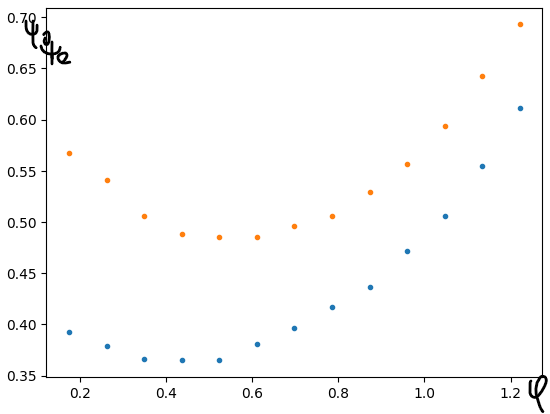
\includegraphics[width=0.4\textwidth]{pi8.png}
    \caption{Зависимость $\psi_o$ и $\psi_e$ от $\varphi_1$}
    \label{fig:example}
\end{figure}

Проверим качество измерений:

\begin{figure}[h]
    \centering
    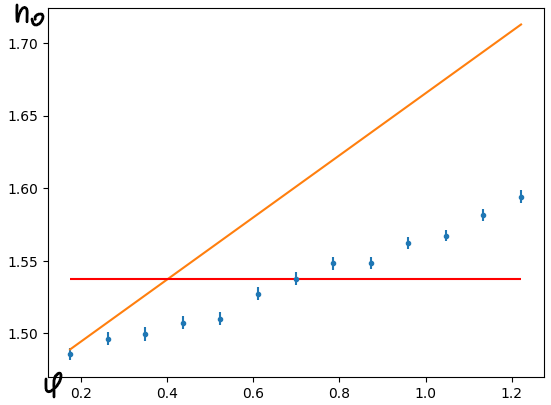
\includegraphics[width=0.4\textwidth]{pi7.png}
    \caption{Зависимость $n_o$ от $\varphi$}
    \label{fig:example}
\end{figure}

Коэффициент наклона должен быть меньше 0.02, но у нас получилось $0.21$, что отличается на порядок от ожидаемой величины.

\par

Найдем показатели преломления по необыкновенной волне:
\[n(\theta) = n_e + (n_o - n_e)cos^2(\theta)\] 

\begin{figure}[h]
    \centering
    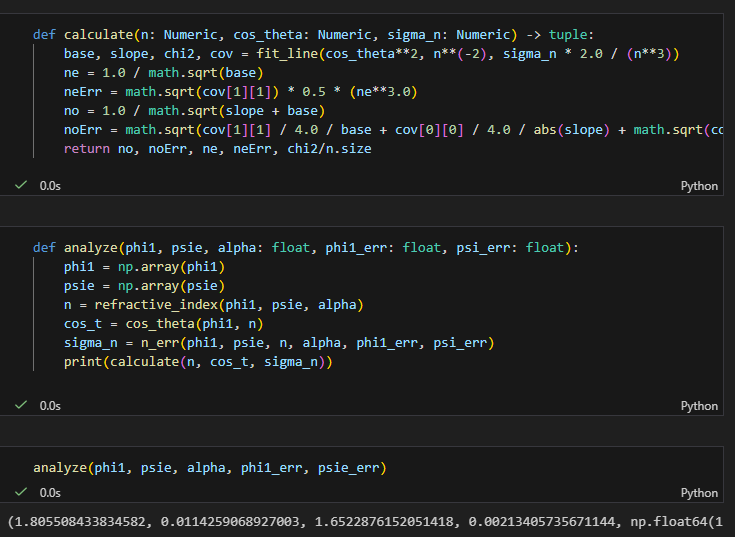
\includegraphics[width=0.4\textwidth]{pi9.png}
    \label{fig:example}
\end{figure}

Получим: $n_0 = 1.806 \pm 0.011$ и $n_e = 1.652 \pm 0.002$ 

\newpage

\section{Вывод:}

Изучили зависимости показателя преломления необыкновенной волны от напрвления в двоякопреломляющем кристалле. Также определили преломляющий угол призмы A и показатель преломления обыкновенной и необыкновенной волн.
В результате значения показателей преломления не сходятся с теоретическими ($n_0 = 1.658$ и $n_e = 1.486$) учетом ошибки. Это может быть связано с тем, что перед выполнением работы мы "покрутили" установку там, где крутить было не нужно. Также на такие 
результаты могла повлиять плохая юстировка системы. При выполнении работы вспомнил, и отработал навык работы с Python и Jupyter Notebook. Использовал современный способ обработки данных в среде разработки.

\section*{Погрешность:}

\begin{figure}[h]
    \centering
    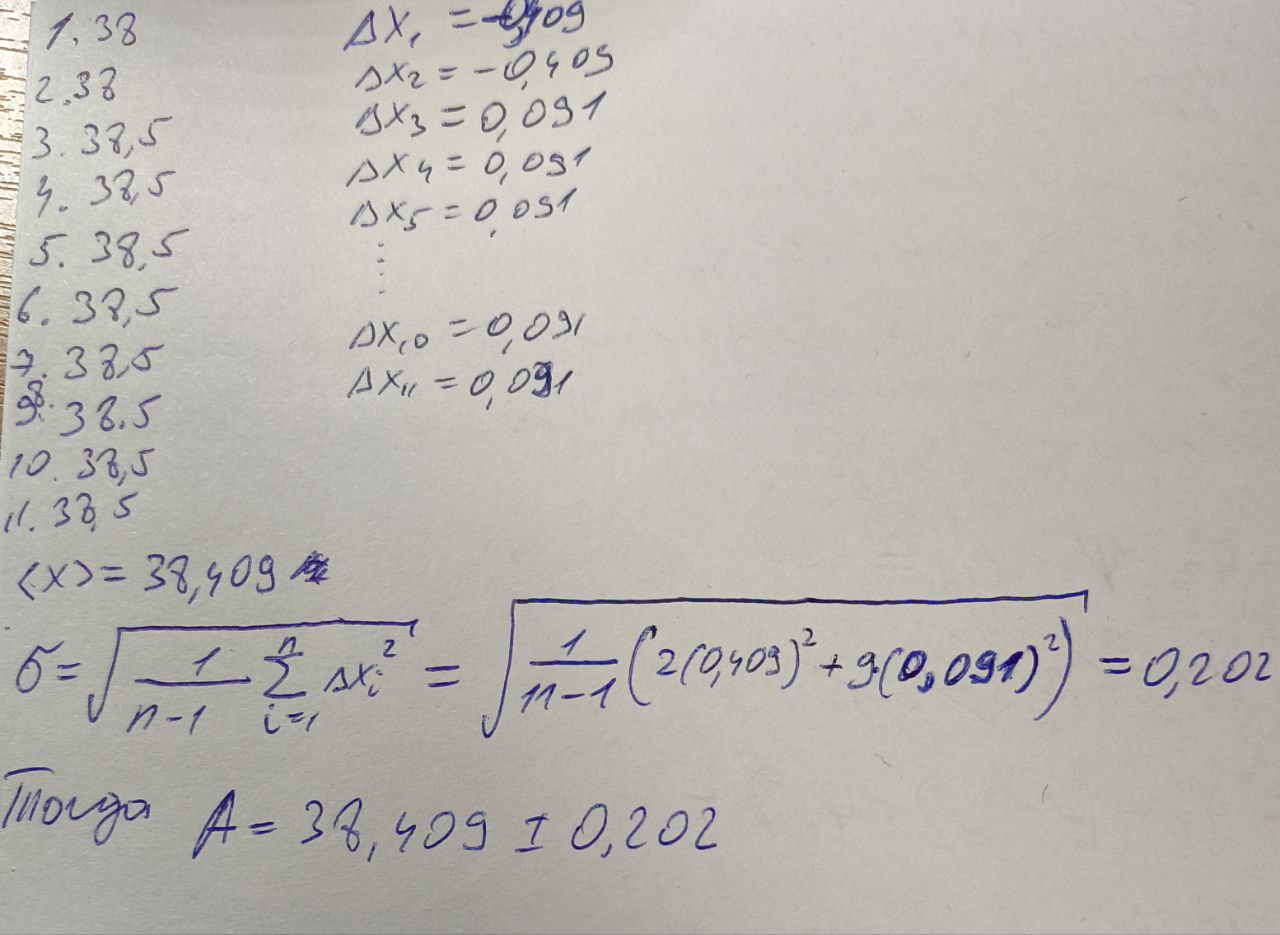
\includegraphics[width=0.7\textwidth]{pi10.jpg}
    \label{fig:example}
\end{figure}

Для величин, посчитанных в работе, погрешности были вычислены с помощью компьютера (см. Jupyter Notebook).

\end{document}